\chapter{Das Neuron}

\section{Struktur einer Nervenzelle}

\begin{figure}[h]
	\centering
		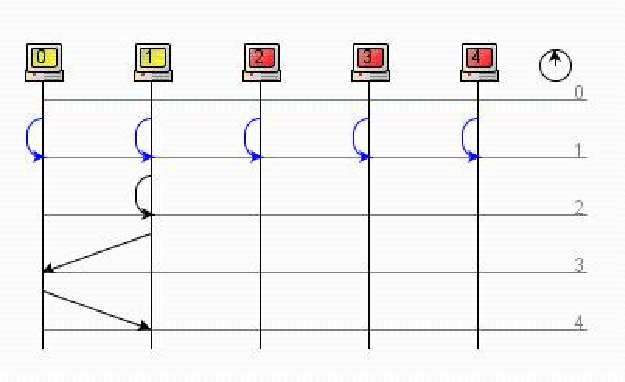
\includegraphics{images/p1ReadSeq.pdf}
\caption{Aufbau einer Nervenzelle}
\small
 1. Die Dendriten leiten
 afferente Signale zum
 2. Soma, dem Zellkörper.
 3. Das Axon leitet ein
 efferentes\footnote{``efferre`` (lat.): hinaustragen, mitnehmen} Nervensignal über präsynaptische Endigungen (Axonterminale) an (häufig weit entfernte)
 Effektoren\footnote{``efficere`` (lat.): bewirken, hervorbringen}
    wie Muskeln und Drüsen oder nachgeschaltete Neuronen
 weiter\footnote{
     Effektoren können wir uns als Endglied der Signalübertragung vorstellen, auch wenn hier wieder interzelluläre Vorgänge stattfinden. Vgl. ``neuromuskuläre Endplatte``\cite[127, Abs. 3]{BCP18}
    } {[SD07:42, Abs. d2]}

\end{figure}



Die eingehende Schnittstelle eines Neurons sind seine \textbf{Dendriten}\footnotetext{
 ``\textgreek{δένδρον} (dendrón)`` (altgriechisch): Baum; einzelne selten länger als 2 mm~\cite[28]{BCP18}. Längere Dendriten finden sich an den kortikalen Pyramidenzellen mit einer Länge von 1 cm {[Eil19:58, ``Polarisierung``]}
}: Baumförmige Fortsätze, die um das \textbf{Soma}\footnote{
  ``\textgreek{σῶμα} (sõma)`` (altgriechisch): Körper; auch \textit{Perikaryon} [RK18:58, ``Aufbau``]. Bezeichnet den Zellkörper und das Stoffwechselzentrum des Neurons mit der eine Grösse von ca. 20 μm~\cite[29]{BCP18}. Zum Vergleich: ein menschliches Haar hat einen Durchmesser von ca. 70 μm, kleine Bakterien bis zu 20 μm.
} herum gelagert sind.
Diese Dendritenbäume~\cite[47]{BCP18} fungieren \textit{postsynaptisch} und empfangen afferente\footnotetext{
  ``afferre`` (lat.): herbeibringen, melden, bringen
} Signale in Form von Neurotransmittern [Eil19:61, ``Synapsen``].
Diese werden von Rezeptoren, die sich an den Enden der Dendriten befinden, aufgenommen.
Oft stehen tausende Neuronen in Verbindung mit den Dendriten eines einzelnen Neurons\footnote{
 das menschliche Gehirn besitzt mindestens $10^{11}$ Neuronen [KSJ+13:175, Abs. 2]
} [SD07, S .42].\\


Die \textbf{Dendriten} leiten Signale weiter an das Soma.
In der Zelle befindet sich das durch die \textit{Neuronenmembran}\footnote{
 Membrandicke ca. 5 nm {[FE19:66, letzter Absatz linke Spalte]}
} von der Umgebung getrennte \textit{Zytosol}, eine salzige, wässrige Flüssigkeit mit einem hohen Anteil von Kalium~\cite[29]{BCP18}\footnote{
 vgl. Ionenkonzentrationen in Tabelle~\ref{tab:ionenkonzentration}
}.
In dem Zytosol eingebettet sind weitere subzelluläre Strukturen mit eigener Membranbegrenzung, die \textit{Zellorganellen} [SD07:8, Abs. 2].\\
Für die weitere Betrachtung ist für uns die Zellmembran und der \textit{transmembranale Transport} von Ionen\footnote{
 hier: der Austausch von Ionen zwischen dem intra- und extrazellulären Raum durch Kanäle und Pumpen. Ion: Ein elektrisch geladenes Atom oder Molekül.
} zur Änderung des Membranpotenzials interessant. In der Nähe des \textbf{Axonhügels}\footnote{
 ca. 20 - 50 µm vom Soma entfernt [Jon19:77, ``Ort der Aktionspotenzialinitiation``]
} entspringt das \textbf{Axon}\footnote{
 ``axon`` (lat.): Achse; Axone können sich im menschlichen Körper über Entfernungen von bis zu über 1m ausstrecken~\cite[28]{BCP18}
}, welches in einer ``salzigen extrazellulären Flüssigkeit mit hoher Leitfähigkeit`` liegt [PCB18:61, Abs. 1]\footnote{
  \textit{Bear et al.} führen das Axon metaphorisch mit einer Telefonleitung zusammen~\cite[43]{BCP18}. Aufgrund der signalempfangenden Eigenschaften und der dünnen Spitzen der Dendriten liegt auch der Vergleich mit ``Antennen`` nahe~\cite[28]{BCP18}
}.
Hier entscheidet sich, ob das Neuron Informationen weiterleitet: Die Summation der durch die postsynaptischen Endigungen eingehenden Signale kann eine Depolarisation\footnote{
  \textit{Depolarisation} bezeichnet die Verringerung des Membranpotenzials von einem negativen Wert auf einen weniger negativen oder gar einen positiven Wert {[RHN+16:812 ``Neurotransmitter und ihre Rezeptoren``]}
} der Membran an dieser Stelle [Eil19:61, ``Soma``] über einen gewissen \textbf{Schwellenwert} bewirken, so das ein \textbf{Aktionspotenzial} ausgelöst wird~\cite[142 f.]{BCP18}, was in den präsynaptischen Endigungen die \textbf{Exozytose}\footnote{
  bezeichnet den Stofftransport aus der Zelle heraus. In den nachfolgenden Abschnitten wird hierdrauf noch näher eingegangen.
} verursacht.


\section{Das Ruhepotenzial}

\subsection{Ionenkonzentrationen und Membranspannungen}\label{sec-ionenkonzentrationen}

Ein Neuron weist \textit{in Ruhe}\footnote{
 vgl. \textbf{Mempranpotenzial}: ``die Spannung an der Nervenzellmembran zu einem beliebigen Zeitpunkt``~\cite[70]{BCP18}; \textbf{Ruhepotenzial}: ``the electrical potential across the membrane in the absence of signaling`` {[KSJ+13:126]}
} eine ungleiche Ionenverteilung zwischen der durch die Zellmembran getrennten intrazellulären Flüssigkeit (IZF: Zytosol) und der extrazellulären Flüssigkeit (EZF) auf.
In der IZF befinden sich mehr positiv geladene Natrium-Ionen ($Na^+$), und im EZF mehr positiv geladene Kalium- und Calcium-Ionen ($Ka^+$ und $Ca^{2+}$) sowie mehr negativ geladene Chlorid-Ionen ($Cl^-$).

{\renewcommand{\arraystretch}{1.5}%
\begin{table} %[hbtp]
 \centering
 \begin{tabular}{l | c | c | c }
  \textbf{Ion} & \textbf{Konzentration EZF (mmol/l)} & \textbf{Konzentration IZF (mmol/l)} & \textbf{Verhältnis} \\
  \hline
  $K^+$      & 5 & 100 & 1 : 20 \\
  $Na^+$     & 150 & 15 & 10:1 \\
  $Ca^{2+}$  & 2 & 0,0002 & 10000 : 1 \\
  $Cl^-$     & 150 & 13 & 11,5 : 1 \\
 \end{tabular}
 \caption{Ionenkonzentration eines Neurons in Ruhe (nach~\cite[75, Abb. 3.15]{BCP18})}
 \label{tab:ionenkonzentration}
\end{table}


Das Membranpotenzial des Neurons wird durch die Verteilung von Ionen in der IZF und EZF bestimmt: In der Membran befinden sich \textbf{Ionenkanäle}, von denen viele \textit{selektiv permeabel}\footnote{
 von ``\textit{permeare}`` (lat.) durchwandern. Diese Kanäle sind nur für bestimmte Ionen durchlässig (\textit{ionenselektiv}). Kaliumkanäle sind durchlässig für $K^+$-Ionen, Natriumkanäle durchlässig für $Na^+$-Ionen usw. (vgl.~\cite[66]{BCP18}).
 Sie können über Änderungen in der Umgebung des Neurons geöffnet oder geschlossen werden, was auch als \textbf{Gating} bezeichnet wird (vgl. {[KSJ+13:108, 2. Abs. rechte Spalte]})
} sind.
Neben den Ionenkanälen existieren auch \textbf{Ionenpumpen}\footnote{
 sog. \textbf{ATPasen}, Kurzform für \textit{Adenosintriphosphasen}: Enzyme, die ATP in ADP und Phosphat aufspalten {[SD07:26, Abs. 2]}) \textbf{QUELLE}
}, die für die Aufrechterhaltung der Ionenverteilung zuständig sind: die $Ca^{2+}$- und $Na^+$-$K^+$-ATPasen sorgen dafür, dass im Neuron laufend  $Ca^{2+}$ und $Na^+$ aus und $K^+$ in die Zelle gepumpt wird [SD07:44]).
Zusammen mit den selektiv permeablen Ionenkanälen entstehen so die Ionenkonzentrationen in Tabelle~\ref{tab:ionenkonzentration}.\\


Wenn auf das Neuron kein \textit{postsynaptisches Potenzial} (PSP) wirkt und das Neuron keinen Impuls abgibt, liegt das Ruhepotenzial $V_r$ der Zelle zwischen -70 mV und -90 mV\footnote{
   vgl. {[SD07:47, Tafel 2.3 A.1]}. \textit{Bear et al.} geben -65 mV an (1 mV = 0,001 V), also wird von einer 40-mal höheren Ionenpermeabilität für $K^+$ gegenüber $Na^+$ ausgegangen (~\cite[74, Exkurs 3.2]{BCP18} und~\cite[70]{BCP18})
}: Das Zytosol weist entlang der Membranoberfläche im IZF eine negative Ladung auf\footnote{
 vgl.~\cite[61]{BCP18}. Das Membranpotenzial $V_m$ ergibt sich als die Differenz der Spannungen $V_{IZF}$ und $V_ezf$, wobei $V_{IZF}$ die Spannung im IZF und $V_{EZF}$ die Spannung im EZF ist. $V_r$ ist dann gleich zu $V_{IZF}$: Wenn die Zelle in Ruhe ist, wird die Spannung im EZF als $0$ definiert {[KSJ+13:127, rechte Spalte, Abs. 2]}.
}.
Diese \textit{Membranspannung} $V_m$ wird durch eine ungleiche Ionenverteilung bewirkt [FE19:66, ``Diffusionspotenzial – elektrische Spannung über der Zellmembran``]), verursacht durch die Ladung der Teilchen im IZF und EZF in Membrannähe\footnote{
 ``Die negativen Ladungen im Inneren des Neurons und die positiven Ladungen außerhalb des Neurons ziehen sich in Richtung Zellmembran gegenseitig an, {[...]} Dementsprechend ist die negative Nettoladung im Inneren der Zelle nicht gleichmäßig im Cytosol verteilt, sondern an der Innenseite der Membran lokalisiert.``~\cite[72, Punkt 2]{BCP18}
}.


\begin{figure}[h]
 \centering
 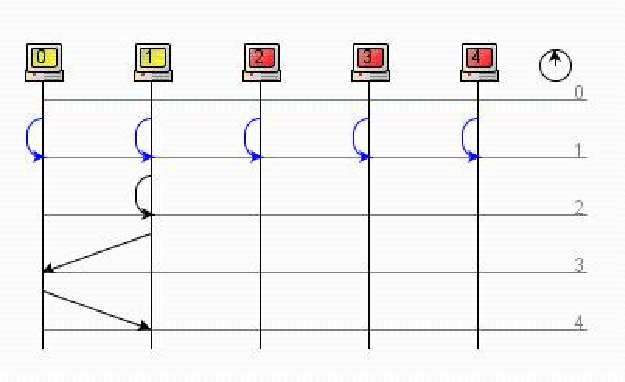
\includegraphics{images/p1ReadSeq.pdf}
 \caption{Ionenverteilung im Zytosol und der EZF}
 \small
 Aufgrund der elektrostatischen Anziehungskraft ziehen sich Anionen (neg. geladen) und Kationen (pos. geladen) in der Nähe der Membran gegenseitig an, es kommt zu einer negativen Spannung in Membrannähe (zwischen -70 mV -90 mV in Ruhe).
\end{figure}

In Ruhe ist die Leitfähigkeit der Membran für $Na^+$ gering, für $K^+$ hingegen hoch [SD07:44 f.].
$K^+$-Ionen folgen ihrem Konzentrationsgradienten\footnote{
 unter der Diffusion (``\textit{diffundere}`` (lat.): zerstreuen, ausbreiten) von Molekülen versteht man ihr Bestreben, entlang eines Konzentrationsgradienten (auch: Konzentrationsgefälles) einen Ausgleich der Konzentrationsunterschiede zu erreichen. Moleküle in hoher Konzentration diffundieren dann in die Bereiche mit niedriger Konzentration: In den hier betrachteten Beispielen diffundieren bspw. $K^+$-Ionen, bis das Gleichgewichtspotenzial erreicht ist.
} und gelangen über die Ionenkanäle in den EZF, bis die Potenzialdifferenz entlang der Neuronenmembran ausströmende $K^+$-Ionen zurückhält: Wenn diese Differenz den Konzentrationsgradienten für $K^+$ kompensiert, erhält man das \textbf{Gleichgewichtspotenzial}\footnote{
 vgl. ~\cite[72]{BCP18} sowie [SD07:44 f.]. \textit{Kandel et al.} schreiben hierzu:
 ``the equilibrium potential of any ion that is present on both sides of a membrane permeable to that ion`` {[KSJ+13:130, letzter Abs., linke Spalte]}
}.
Das Wert des Membranpotenzial nähert sich dem Wert des Gleichgewichtspotenzials desjenigen Ions an, für den die Membran besonders permeabel ist [KSJ+13:145, Ende] $(S1.1)$.\\
Das Gleichgewichtspotenzial lässt sich für individuelle Ionen mit der Nernst-Gleichung\footnote{
 vgl. {[FE19:67, ``Nernst-Gleichung``]}.
} ermitteln (s. Gleichung~\ref{eq:gl-nernst} sowie Tabelle~\ref{tab:nernstkonstanten}):\\

\textit{Bear et al.} definieren~\cite[74, Exkurs 3.2]{BCP18}:
\begin{equation}
E_{Ion} = 2,303  \times \begin{matrix} RT \\ \hline zF \end{matrix} \times log_{10} \times \begin{matrix} [Ion]_{EZF} \\ \hline [Ion]_{IZF} \end{matrix}
\label{eq:gl-nernst}
\end{equation}



  {\renewcommand{\arraystretch}{1.5}%
\begin{table} %[hbtp]
 \centering
 \begin{tabular}{l |l }
  \textbf{Variable / Konstante} & \textbf{Bedeutung}  \\
  \hline
  $E_{ion}$            & Gleichgewichtspotenzial für das jeweilige Ion \\
  $R$                  & Gaskonstante \\
  $T$                  & absolute Temperatur \\
  $z$                  & Ladungszahl des Ions \\
  $F$                  & Faraday-Konstante \\
  $[Ion]_{EZF}$        & Ionenkonzentration \textbf{ausserhalb} der Zelle \\
  $[Ion]_{IZF}$        & Ionenkonzentration \textbf{innerhalb} der Zelle \\
 \end{tabular}
 \caption{Nomenklatur Nernst-Gleichung}
 \label{tab:nernstkonstanten}
 \small
  $E$ steht für \textit{Equilibrium}: ``Gleichgewicht``; \textit{Faraday-Konstante}: elektrische Ladung eines Mols einfach geladener Ionen; 1 Mol = $6.02214076e10^{23}$ Teilchen

\end{table}

\noindent
Für eine Körpertemperatur von 37° lässt sich die Nernst-Gleichung für das Gleichgewichtspotenzial $E_K$ wie folgt vereinfachen:

\begin{equation}
 E_{K} = 61,54 mV  \times log_{10} \begin{matrix} [K^+]_{EZF} \\ \hline [K^+]_{IZF} \end{matrix}
 \label{eq:gl-nernst-reduced-start}
\end{equation}

\noindent
Mit den Werten aus Tabelle~\ref{tab:ionenkonzentration}  ergibt sich somit


\begin{equation}
E_{K} = 61,54 mV  \times log_{10} \begin{matrix} 1 \\ \hline 20 \end{matrix} = -80 mV
\label{eq:gl-nernst-reduced-end}
\end{equation}

\noindent
Um auf $(S1.1)$ zu schliessen und $V_m$ zu berechnen müssen die Ionen mitberücksichtigt werden, für die die Membran permeabel ist.
Dazu kann die \textbf{Goldman-Gleichung}\footnote{
 s. \ref{appendix:goldman}
} genutzt werden:

\begin{equation}
V_{r} = \begin{matrix} RT \\ \hline F \end{matrix}  \times ln \begin{matrix}
  P_{Na} \space  \times \space [Na^+]_{EZF} \space + \space P_{K} \space  \times \space [K^+]_{EZF} \space + \space P_{Cl} \space  \times \space [Cl^-]_{IZF}  \\ \hline
  P_{Na} \space  \times [Na^+]_{IZF} \space + \space P_{K} \space  \times \space [K^+]_{IZF} \space + \space P_{Cl} \space  \times \space [Cl^-]_{EZF}
\end{matrix}
\label{eq:gl-goldman}
\end{equation}

Ein weiteres Merkmal der Membran, auf das wir später zurückgreifen werden, ist die \textit{elektrische Leitfähigkeit} $g_{Ion}$; für sie gilt, dass sie proportional zu der Anzahl der offenen Ionenkanäle $N_{Ion}$ ist~\cite[93]{BCP18}.

\section{Das Aktionspotenzial}

\subsection{Eigenschaften des Aktionspotenzials}

In Ruhe ist die Ladung in der IZF negativ, in der EZF positiv.
Durch eine schnelle Umkehrung dieser Verhältnisse ist eine Nervenzelle dazu in der Lage, ein \textit{Signal} auszulösen~\cite[86]{BCP18}.
Damit solch ein Impuls ausgelöst werden kann, bedarf es eines \textbf{Aktionspotenzials}: Wir wir im folgenden sehen werden, ist die Entstehung eines Aktionspotenzials auf Ionenbewegungen durch Kanäle zurückzuführen, die durch die Veränderung des Membranpotenzials geöffnet oder geschlossen werden~\cite[96]{BCP18}.

 \textit{Kandel et al.} führen 4 wichtige Eigenschaften des Aktionspotenzials auf [KSJ+13: 148, Abs. 2 f.]:
\begin{enumerate}
 \item Es gibt einen \textbf{Schwellenwert} für die Auslösung des Potenzials.
 \item Das Aktionspotenzial ist ein \textbf{Alles-oder-nichts} Ereignis.
 \item Das Aktionspotenzial wird ohne Verlust weitergeleitet.
 \item Nach dem auslösen des Aktionspotenzial kommt es zu einer \textbf{Refraktärzeit} , in der zunächst kein weiteres Aktionspotenzial ausgelöst werden kann (\textbf{absolute Refraktärzeit}), und dann ein stärkeres Signal benötigt wird, um das Aktionspotenzial auszulösen (\textbf{relative Refraktärzeit}).
\end{enumerate}


\subsection{Auslösung eines Aktionspotenzials}

Das Aktionspotenzial wird über das Axon weitergeleitet. Das Axon - die Nervenfaser - besteht aus einem zylindrischen Zytoplasmaschlaucch und ist von einer Plasmamembran umgeben [Jon19:73, ``Elektrischer Signalfluss im biologischen Kabel``].

Die \textbf{Initiationszone}~\cite[111]{BCP18} des Aktionspotenzials ist der Axonhügel. Hier findet sich eine besonders dichte Anhäufung von spannungsabhängigen $Na^+$-Kanälen\footnote{
 pro Quadratmikrometer (µm²) kann eine Membran viele tausend Natriumkanäle enthalten~\cite[99]{BCP18}
}, deren Aktivierungskurve um ca. 10 mV zu den negativen Membranpotenzialen verschoben ist, was die Initiierung des Signals begünstigt [Jon19:77, ``Mechanismen der Aktionspotenzialinitiation und ihrer räumlichen Präferenz``)].

Damit ein Aktionspotenzial ausgelöst werden kann, muß die Membran nahe der Initiationszone über ihren \textbf{Schwellenwert} \footnote{
 ``das kritische Niveau der Depolarisation, das überschritten werden muss, um ein Aktionspotenzial auszulösen``~\cite[88]{BCP18} oder auch ``Erregungsschwelle`` {[FE19:69, ``Depolarisation``]}
} $V_t$ ( > $V_r$ ) depolarisiert werden~\cite[111]{BCP18}.


 Als Schwellenwert wird das Membranpotenzial bezeichnet, bei dem die Permeabilität für $Na^+$ größer als für $Ka^+$ ist~\cite[103]{BCP18} ($V_r$ ist in Ruhe nahe an $E_K$); $V_t$ liegt bei ca. - 50mV, unabhängig vom Typ des Neurons [Jon19:75].
 Damit sich $V_r$ an $V_t$ nähert, bedarf es einer Erregung der Zelle durch postsynaptische Potenziale [FE19:69 ``Depolarisation`` f.] oder ``eine aus der Umgebung weitergeleitete (elektrotonische) Erregung`` [SD07:46, Abs. 2].

Die Stärke der Erregung der Zelle ist entscheidend für das Auslösen eines Aktionspotenzials. Es muß mehr $Na^+$ in die Zelle einströmen, als $K^+$ aus der Zelle ausströmen kann [FE19:69, rechte Spalte, Abs. 1] (durch die offenen Ruhemembranpotenzialkanäle und Konzentrationsgradientenausgleich der $Na^+$-$K^+$-ATPasen).
Versuche zeigen, daß die Potenzialänderung der Membran in einem Bereich von -80 mV zu -65 mV kaum Änderung bewirkt~\cite[99]{BCP18}. $g_{Ka}$ erhöht sich, aber wenn $V_r$ nicht erreicht wird, bleibt es bei dieser ``lokalen Antwort`` [SD07:46, Abs. 2]. Erst eine Depolarisation der Membran hin über diesen Wert (ab -60 mV gehen die Natrium-Kanäle ein den Offen-Zustand über [FE19:69, rechte Spate, Abs. 2]), kann die \textbf{Initiationsphase} [FE19:68, Abschnitt 6.2] des Aktionspotenzials eingeleitet werden: Es öffnen sich mehr Natrium-Kanäle, und durch die negative Ladung der Membran-Innenseite (IZF) gibt es eine starke elektrochemische Triebkraft für $Na^+$-Ionen~\cite[103]{BCP18}. Die Triebkraft ist zu diesem Zeitpunkt die Differenz des Membranpotenzials $V_m$ und $E_{Ka}$. Bei $-60 mV$ beträgt die Triebkraft\footnote{
 vgl. {[Fak19:39, ``Das elektrochemische Potenzial`` f.]}
}:

 \begin{equation}
  V_m - E_{Na} = -60 mV - 61,54 mV = -121,54 mV
  \label{eq:gl-triebkraft}
 \end{equation}


Da sich $g_{Ka}$ erhöht durch zunehmende Öffnung der Natrium-Kanäle  [Fak19:46, ``Gating von Kationenkanälen`` ff.], strömen aufgrund der hohen Triebraft für $Na^+$ mehr $Na^+$ Ionen in das Zellinnere. Es kommt zu einem \textbf{Rückkopplungseffekt} , denn die zunehmend weniger negative Membranspannung öffnet weitere Natrium-Kanäle, die Leitfähigkeit der Membran wird weiter erhöht und es kommt zu einem exponentiellen Anstieg der $Na^+$-Konzentration in der IZF. Der ``explosionsartige`` Natriumeinstrom bewirkt die Depolarisation der Membranspannung und das Aktionspotenzial wird ausgelöst [FE19:69, ``Depolarisation`` f.]\footnote{
s. \ref{appendix:aktionspotenzial}
}.

Die Stärke des Signals selber ist unabhängig von dem Wert, zur überschwelligen Reizung des Neurons geführt hat: Amplitude und Zeitverlauf des Signals im Axon relativ unabhängig von Intensität und Dauer des Reizes [Jon19:75, ``Aktionspotenziale bei überschwelliger Reizung``]. Entweder kommt es zu einem Aktionspotenzial, oder es bleibt bei der o.g. lokalen Antwort. Aus diesem Grund funktionieren Aktionspotenziale nach dem \textbf{``Alles-oder-Nichts-Prinzip``}~\cite[89]{BCP18}\footnote{
 ``Im Computerzeitalter bezeichnet man das axonale Aktionspotenzial auch als 'digitales' Signal.`` {[Jon19:75, ``Aktionspotenzial bei überschwelligger Reizung``]}. \tetxit{Frank} bietet eine Übersicht über die Erforschung des Alles-oder-Nichts-Prinzip in [Fra94]. Dort wird \textit{Lucas} erwähnt, der 1905 in {[Luc05]} die Kontraktionen von Muskelfasern unter diesem Gesichtspunkt untersucht hat {[Fra94:210]}
}:

\blockquote[{[KSJ+13:157, rechte Spalte, Abs. 2]}]{
 ``A fraction of a millivolt can be the difference between a subthreshold stimulus and a stimulus that generates a full-sized action potential.``
}

\subsection{Signalweiterleitung über das Axon}

Kurz nach der Aktionspotenzialbildung befinden sich daran beteiligte Membrane in der Refraktärphase, ihre $Na^+$-Kanäle sind inaktiviert. 
Somit pflanzt sich das Aktionspotenzial nur in eine Richtung fort\footnote{
  \textit{Bear et al.} verweisen auf \textit{antidrome} Fortleitung, die in Experimenten ausgelöst werden kann~\cite[106]{BCP18}
} ( \textit{orthodrome} Fortleitung)~\cite[106]{BCP18}.
Die Fortleitung geschieht in Richtung der Axonterminal, wo sich die präsynaptischen Endigungen befinden und das elektrische Signal in chemische Signale umgewandelt werden.

\vskip 1.6in


\pagebreak

\section{Synaptische Übertragung und Integration}


\subsection{Synaptische Übertragung}\label{synaptischeuebertragung}
Neben elektrischen Synapsen, bei denen der Signalaustausch durch einen direkten Stromfluss über sogenannte \textit{gap junctions} und deren ionenleitfähige Verbindungen\footnote{
 \textit{Konnexone} sind Zell-Zell-Verbindungen {[SD07:50, ``Synaptische Übertragung``, Abs. 2]}
} passiert~\cite[119]{BCP18}, erfolgt die Signalweiterleitung im Gehirn überwiegend auf chemische Weise~\cite[121 ff.]{BCP18}.

Chemische Synapsen sind nicht direkt miteinander verbunden. 
Zwischen ihnen existiert ein Spalt, der ca. 20-40 nM breit ist [KSJ+13:184, rechte Spalte, Abs. 1], in der sich eine ``Matrix aus extrazellulären Proteinen``\footnote{
 lies: \textit{extrazelluläre Matrix}. Hierbei handelt sich um den Gewebeanteil im \textit{Interzellularraum}, also der Raum ausserhalb der Zellen: ``The extracellular matrix {[...]} surrounds all connective tissue cells providing mechanical support and physical strength to tissues, organs and the organism as a whole`` {[AHH+98:3, Abs. 2]}
} befindet, die den Synapsenspalt überbrückt~\cite[122]{BCP18}.
Die Übertragung von Signalen erfolgt über Exozytose: Botenstoffe (\textit{Neurotransmittern}) diffundieren aus den präsynaptischen Endigungen in diesen Spalt~\cite[122]{BCP18}, und verschiedene Typen von Rezeptoren an den postsynaptischen Endigungen wandeln die Botenstoffe in hemmende oder erregende Signale um, die dann von der postsynaptischen Zelle nach dem Alles-oder-Nichts-Prinzip integriert werden.

Die durch das Aktionspotenzial ausgelöste Depolarisation der Membran an den Axonterminalen bewirkt eine Öffnung spannungsgeladener Calcium-Canäle [KSJ+13:184, rechte Spalte, Abs. 2].
Durch die ungleiche $Ca^{2+}$ Ionenkonzentration zwischen der EZF und IZF (10.000 : 1:Tabelle~\ref{tab:ionenkonzentration}) entsteht eine hohe Triebkraft für $Ca^{2+}$: Nach Gleichung~\ref{eq:gl-nernst} ergibt sich für das Gleichgewichtspotenzial für $Ca^2+$

\begin{equation}
 E_{Ca^{2+}} = 123,08 mV
 \label{eq:gl-eqca2}
\end{equation}



\pagebreak

und bei einem Membranpotenzial von $V_m \sim 20 mV$ durch Depolarisation liegt die Triebkraft für $Ca^{2+}$ bei $\sim -100 mV$:

\begin{equation}
 V_m - E_{Ca^{2+}} = 20 mV - 123,08 mV = -103,08 mV
 \label{eq:gl-triebkraftca2}
\end{equation}


Die Calcium-Ionen strömen in das Innere der Zelle und lösen die Exozytose von \textbf{synaptischen Vesikeln}\footnote{
 ``\textit{vesicula}`` (lat.): ``Bläschen``
} aus, kleine, mit einer Membran von der IZF getrennte Strukturen von etwa 50 nm Durchmesser, die mit Neurotransmittern gefüllt sind~\cite[1000]{BCP18}.
Im \textit{synaptischen Endknöpfchen} befinden sich 100-200 von diesen Bläschen, die jeweils tausende Moleküle eines Neurotransmitters beinhalten [KSJ+13:184, rechte Spalte, Abs. 2``].

Der Calciumeinstrom in die präsynaptische Endigung löst die Verschmelzung dieser Bläschen mit der Zellmembran des Endknöpfchens an der sogenannten \textbf{aktiven Zonen}\footnote{
 \textit{Bear et al.} beschreiben das Aussehen der aktiven Zone als ``ein Feld winziger Pyramiden``~\cite[123]{BCP18}
} aus: Ein spezialisierter Abschnitt der Membran, der direkt gegenüber der \textbf{postsynaptischen Dichte}\footnote{
 [RK18] spricht von direkter Einwirkung (inotrop) und indirekter Einwirkung (metabotrop) [RK18:134, rechte Spalte, Abs. 2]
} liegt, der Abschnitt der postsynaptischen Endigung, in der sich die Rezeptoren [BLS19:95, ``Die Struktur chemischer Synapsen`` ff.] befinden.
Kurz nach Beginn der Transmitterübertragung über den synaptischen Spalt findet die \textbf{Endozytose} statt, ein Recyclingprozess, in dem die individuellen Vesikelmembranen wiederhergestellt und mit Neurotransmitter erneut aufgefüllt werden~\cite[133]{BCP18}.


\subsection{Synaptische Integration}

Die Neurotransmitter eines einzelnen Vesikels lösen einen minimalen exzitatorischen oder inhibitorischen postsynaptischen Strom aus (\textbf{mEPSC} bzw. \textbf{mIPSC}, \textit{miniature excitatory / inhibitory postsynaptic current}) . 
EPSCs und IPSCs setzen sich aus einzelnen dieser mEPSC bzw. mIPSC zusammen und bilden die kleinste Einheit der postsynaptischen Ströme, weshalb man sie als \textit{Quanten} bezeichnet [BLS19:97, ``Quantale Transmitterfreisetzung`` ff.]. 
Da EPSPs ein Vielfaches des Quantums sind, ``das die Menge an Transmitter in einem einzigen Vesikel und die Anzahl der postsynaptischen Rezeptoren an der Synapse widerspiegelt``, nennt man sie ``gequantelt``\footnote{
 Mit Hilfe der \textbf{Quantelungsanalyse} läßt sich die Anzahl der an einer synaptischen Übertragung beteiligten Vesikel bestimmen~\cite[142]{BCP18}.
}[PCB18:142, Abs. 1].

Wesentlich für die Entstehung eines neuen Aktionspotenzials in der postsynaptischen Zelle ist die Verrechnung der räumlich oder zeitlich eintreffenden Signale. 
Hierbei ist die \textbf{räumliche Summation} die Integration von vielen fast gleichzeitig eintreffenden Signalen mehrerer präsynaptischer Zellen, die sich in der Folgezelle zu einem EPSP aufaddieren [BLS19:101, ``Räumliche Summation``]. 
Unter der \textbf{zeitlichen Summation} versteht man die in gewissen Abständen von ein und derselben Synapse hintereinander eintreffenden EPSPs, die jeweils  das Membranpotenzial für nachfolgende Signale zum Schwellenwert hin verschieben\footnote{
 vgl.~\cite[142]{BCP18} sowie [BLS19:101, ``Zeitliche Summation``]
}.
Ob der Schwellenwert der postsynaptischen Zelle überschritten werden kann ist auch abhängig von dem Abstand der Synapsen von der Initiationszone und den Eigenschaften der dendritischen Membran.

So kann die EPSP-Amplitude kleiner werden, wenn Strom auf dem Weg zu dem Axonhügel durch die Membran verloren geht~\cite[142 f.]{BCP18}\footnote{
 \textit{Bear et al.} vergleichen die Dendriten mit einem löchrigen Gartenschlauch~\cite[143]{BCP18}
}.

Zu berücksichtigen ist natürlich auch der Einfluss inhibitorischer Synapsen auf die Zelle: Inhibitorische ``Eingaben``, die hyperpolarisierend wirken, werden von den exzitatorischen Eingaben subtrahiert\footnote{
 \textit{Bear et al.} stellen in~\cite[146, Exkurs 5.6]{BCP18} die Bedeutung inhibitorischer Synapsen anschaulich dar.
} [KSJ+13:225, rechte Spalte, Abs. 2].


Das Zusammenspiel zwischen exzitatorischen und inhibitorischen Synapsen wird auch durch das \textbf{Umkehrpotential} bestimmt. 
Wie wir bei der Entstehung des Aktionspotenzials gesehen haben, transportieren spannungsgesteuerte Ionenkanäle stets entlang des elektrochemischen Gradienten [BLS19 S. 39 ``Das elektrochemische Potenzial`` f.]. 
Die Membran sei zur Vereinfachung nur permeabel für ein Ion, es gelte weiterhin $V_m < E_{Ion}$: Die Stromrichtung für das Ion ist einwärts IZF (vgl $Gl1.1$). Ist die Triebkraft positiv wegen $V_m > E_{Ion}$, strömt das Ion auswärts EZF. Wenn allerdings

\begin{equation}
V_m - E_{Ion} = 0
\end{equation}

dann gilt:

\begin{equation}
V_m = E_{Ion}
\end{equation}

In diesem Fall entspricht die Membranspannung dem Gleichgewichtspotenzial des Ions - es findet keine Nettoionenbewegung statt.\\

Der Wert für $V_m$, bei dem die Differenz zwischen $V_m$ und $E_{Ion}$ bei $0$ liegt, wird das _Umkehrpotenzial_ $V_{rev}$ genannt, weil hier ein Vorzeichenwechsel stattfindet: Je nachdem, in welche Richtung sich $V_m$ ändert, ändert sich auch die Richtung des Stroms. 
Für ionenspezifische Kanäle entspricht das \textit{Umkehrpotenzial} ihrem \textit{Gleichgewichtspotenzial} [SBB+12:95, ``Hyperpolarization or Depolarization`` f.].\\

Sobald eine Membran permeabel für mehr als ein spezifisches Ion ist, muss nach [KSJ+13] die relative Leitfähigkeit der Membran für diese Ionen sowie deren Gleichgewichtspotenziale zur Bestimmung des Umkehrpotenzials berücksichtigt werden. 
Für die ACh-Rezeptoren an der motorischen Endplatte\footnote{
 chemische Synapse, die Erregungen an eine Muskelfaser weiterleitet [SD07:56, ``Motorische Endplatte``]
}, die für $Na^+$ und $K^+$ permeabel sind, folgt damit, dass die Summe ihrer Ströme am Umkehrpotenzial $V_{rev} = 0$ sein muss:

\begin{equation}
I_{Ka} + I_{Na} = 0
\end{equation}

Da der Membranstrom $I_{Ion}$ gleich dem Produkt der Membranleitfähigkeit und der elektrochemischen Triebkraft für dieses Ion ist~\cite[93]{BCP18}, also

\begin{equation}
I_{Ion} = g_{Ion} * (V_m - E_{Ion})
\end{equation}

liefert Ersetzen die Gleichung

\begin{equation}
g_{Na} * (V_m - E_{Na}) = g_{K} * (V_m - E_{K})
\end{equation}

Da am Umkehrpotential $V_{rev} = V_m$ gilt, können wir $V_m$ durch $E_{rev}$ ersetzen und danach auflösen, was zur folgenden Gleichung führt (vgl. [KSJ+13:196, Box 9-1 f.]):

\begin{equation}
E_{rev} = \begin{matrix}
            E_{Na} \space * \space (g_{Na} \space / \space g_{K}) \space + \space E_{K}  \\ \hline
            (g_{Na} \space / \space g_{K}) \space + 1
\end{matrix}
\end{equation}

Die ACh-Rezeptoren haben an der Endplatte eine relative Leitfähigkeit für $Na^+:K^+$ von $1,8$, für die Gleichgewichtspotenziale gilt $E_{Na} = +55 mV$ und $E_{K} = -100 mV$; somit folgt nach Einsetzen $E_{rev} = 0mV$ [BLS19:100, ``Acetylcholnrezeptoren``].
Wenn nun das Membranpotenzial vor der Einwirkung von ACh $< 0mV$ ist, bewirkt ein Öffnen der Ionenkanäle einen Strom einwärts IZF, um $V_m$ auf $0$ zu bringen (Depolarisation); im umgekehrten Fall $V_m > 0$ fließen Ionen auswärts zu EZF, und es findet eine Hyperpolarisation statt~\cite[136, Exkurs 5.4]{BCP18}.\\

Im Allgemeinen gilt, das an erregenden Synapsen unspezifische Kationenkanäle öffnen, deren Umkehrpotential im Bereich von $0mV$ liegt: Hier kommt es zu einer Depolarisation (EPSP). An hemmenden Synapsen öffnen $Cl^-$- oder $K^+$-Kanäle und es gilt dort $V_{rev} \leq V_r$, wonach es meist zu einer leichten Hyperpolarisation kommt [BLS19:100, ``9.3.2 Umkehrpotenzial`` ff.].\\

Die Verrechnung von EPSP und IPSP erfolgt nicht ausschließlich linear durch Summation - inhibitorische Synapsen können auch für einen ``Kurzschluss`` sorgen und somit ein EPSP um ein Vielfaches verkleinern [Sil03:477, ``Shunting inhibitory conductances`` f.]. Man spricht dann von einer \textit{Kurzschlusshemmung} (\textbf{shunting inhibition})\footnote{
 s. \ref{appendix:shuntinginhibition}
}.






% \[\^(.*?)\] %footnotemark regex
%  _(.*?)_ % textit
%  \*\*(.*?)\*\* % textbf
% [(.*?)] % [$1]